\chapter{Nowa metoda oceny procesu gojenia ścięgna Achillesa}
\label{NewMethod}

%ATRS \cite{Kearney2012}, VISA-A \cite{Robinson2001} or FAOS \cite{Roos2001} - dorzuć do biomechaniki.

%	Medical Imaging - especially Magnetic Resonance Imaging (MRI) and Ultrasonography (US) - is one of the most common technique that nowadays is used to monitor soft tissues. Some papers e.g.  \cite{Khan2003, Ibrahim2013} indicate the advantage of MRI over US showing that MRI appearance can be easier associated with the clinical outcomes. Despite this, US also present in e.g. \cite{vanSchie2009, PradoCosta2018} as a valuable technique for the soft tissues properties investigation, yet technical issues and lack of standardization limits its use.} - dorzuć do USG/MRI

% Poniżej powinno być opisane tylko RM i krótkie uzasadnienie, potem dane tylko RM i jedna krótk sekcja z USG.

W tym rozdziale zostanie zaprezentowana autorska propozycja metody oceny procesu gojenia się ścięgna Achillesa bazująca na badaniach obrazowych. W szczególności przedstawiony zostanie ilościowy opis, umożliwiający w zobiektywizowany sposób ocenę morfologii tkanek widocznych w obrazach Rezonansu Magnetycznego i Ultrasonografii. Finalnie zostanie również zaproponowane nowatorskie podejście do automatycznego wyliczania wskazanych w opisie procesu parametrów, co jest najważniejszym osiągnięciem całości tej pracy. 

Wskazana automatyzacja została przez autora wykonana dla danych z Rezonansu Magnetycznego, które zostały przez specjalistów wskazane jako klinicznie bardziej istotne niż USG. Niemniej jednak dane Ultrasonografii zostały również przeanalizowane pod kątem wartości dodanej do całego proponowanego procesu.  

W chwili pisania tej pracy nie istnieje wedle najlepszej wiedzy autora podejście umożliwiające zobiektywizowany i co ważniejsze automatyczny sposób oceny badań obrazowych prezentujących gojące się ścięgno Achillesa. Stąd implikacje dotyczące trudności z integracją subiektywnych interpretacji ze skalami testów funkcjonalnych takich jak ATRS i w rezultacie zmniejszona efektywność całego procesu oceny rehabilitacji. 

Podczas próby rozwiązania wskazanego problemu autor tej pracy w szczególności chce skupić się na dwóch aspektach. Pierwszym z nich jest jakość generowanej automatycznie oceny odniesiony do jakości wzorca tj. oceny doświadczonego radiologa. Drugim natomiast jest czas akwizycji danych, a zatem wybór praktycznego protokołu, który zapewni możliwie krótki udział pacjenta w badaniu. W obu przypadkach celem jest poszukiwanie punktu optimum, w którym maksymalizowana będzie jakość oceny, a minimalizowany czas, zarówno radiologa jak i pacjenta, niezbędny do wykonania koniecznych czynności. Szczegóły podejścia zostały opisane w kolejnej sekcji.


\section{Metodyka}

W tej sekcji zostanie szczegółowo opisana proponowana metoda automatycznej oceny procesu gojenia się ścięgna Achillesa widocznego w badaniach obrazowych Rezonansu Magnetycznego. Dodatkowo scharakteryzowany zostanie zbiór danych, który posłużył do opracowania rozwiązania, jak również ankieta walidacyjna stanowiąca wzorzec odniesienia dla przedstawionej metody. 

Autor tej pracy, w proponowanym podejściu skorzystał z metod widzenia komputowego, a dokładniej z fuzji algorytmów sztucznej inteligencji i przetwarzania obrazów. W kontekście tej pracy, pierwsze znajdują swoje zastosowanie do ekstrakcji wektora cech dla danej reprezentacji obrazowej. Drugie, pozwalają uwzględnić wiedzę dziedzinową w procesie numerycznej oceny.

W przypadku algorytmów sztucznej inteligencji zastosowano  opisane w Rozdziale \ref{CNNs} konwolucyjne sieci neuronowe, a dokładniej AlexNet, GoogLeNet (inceptionV3) i ResNet-18. W pierwszej kolejności wykonane zostało szkolenie podanych sieci dla problemu binarnej klasyfikacji tj. odróżniania obrazów chorego od zdrowego ścięgna. Następnie część klasyfikująca została usunięta z topologii sieci, pozostawiając ekstraktor cech z parametrami zoptymalizowanymi pod kątem wydobycia istotnej informacji opisującej różnice między zdrową i chorą tkanką. Na tak otrzymanym wektorze, przeprowadzono redukcję wymiarowości z wykorzystaniem metody PCA (zob. \ref{DimReduction}). W wyniku przeprowadzonych eksperymentów, ostatecznie zdecydowano się uwzględnić 200 pierwszych czynników głównych w końcowym rozwiązaniu.

W przypadku metod przetwarzania obrazów zastosowano obliczenia cech z wydzielonego przez specjalistę radiologa ROI (od ang. \textit{Region of Interest}) reprezentującego tkanki otoczone ościęgnem. Sumarycznie wyliczono 46 klasycznych cech obrazowych, w tym pole powierzchni ROI, 9 cech opisujących statystykę wartości pikseli i 36 cechy Haralick'a opisujące teksturę (zob. \cite{Haralick1973}). W ramach statystyk scharakteryzowano: min, max, średnią, odchylenie standardowe, skośność, kurtozę, 25-percentyl, medianę oraz 75-percentyl. Natomiast w ramach cech Haralick'a: drugi moment kątowy, kontrast, korelacja, wariancja, odwrotny moment różnicowy, suma średnich, suma wariancji, suma entropii, entropia, różnica wariancji i maksimum prawdopodobieństwa. Cechy Haralick'a wyliczono dla 3 dystansów separacji \textit{d}=1,5,10. Dokładna metoda selekcji powyższych cech została przedstawiona w pracy  \cite{Nowosielski17}.  

Spośród tak wyliczonych 246 cech dokonano selekcji metodą LASSO (zob. [opis]). W rezultacie dla wszystkich ocenianych parametrów uzyskano optymalną mieszaninę poniżej 20 cech ekstrahowanych z wykorzystaniem sieci konwolucyjnych oraz klasycznych metod obrazowych. Wybrane predyktory posłużyły do szkolenia algorytmu meta-regresji, przy użyciu którego wykonana została fuzja.   

Końcowa ocena badania została wykonana następującą metryką $H$ zaproponowaną przez autora tej pracy:
\begin{equation}
\label{ecq:H}
H = TM(R(x_1), R(x_2),..., R(x_n))
\end{equation}
gdzie $TM$ jest średnią trymowaną z marginesami 2.5\%, a $R(x_i)$ jest wynikiem regresji obliczonym dla przekroju osiowego $x_i$, gdzie $i$ to indeks przekroju w trójwymiarowym badaniu RM.

Schemat powyższej metody został zaprezentowany na Fig. \ref{fig:net}. 
\begin{figure}[h!]
	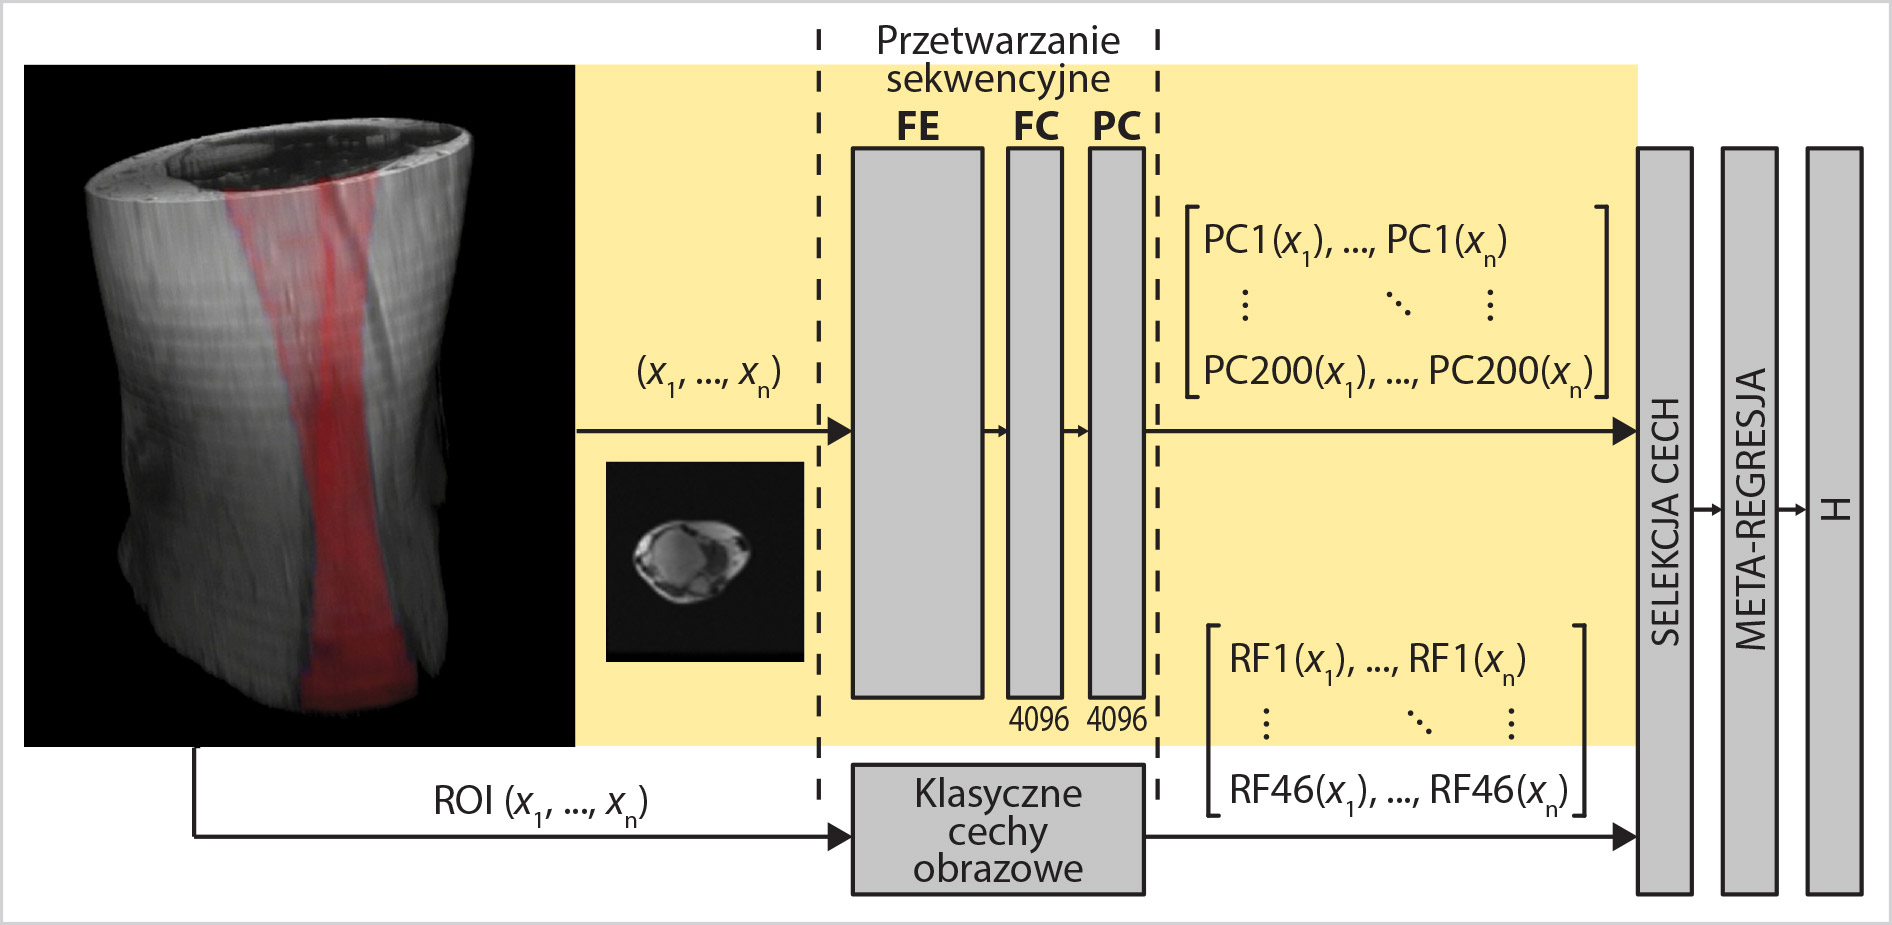
\includegraphics[width=\textwidth]{figures/net.jpg}
	\caption{Schemat automatycznej metody oceny procesu gojenia się ścięgna Achillesa.} \label{fig:net}
\end{figure}
W ogólnym ujęciu trójwymiarowe badanie RM dzielone jest na pojedyncze przekroje osiowe, które stanowią dane wejściowe do oznaczonej na żółto części opartej o metody głębokiego uczenia się. Początkowo dane przetwarzane są prze ekstraktor cech sieci AlexNet wybranej w wyniku eksperymentów (FE). Następnie wstępnie grupowane są z wykorzystaniem warstwy fully connected (FC) i poddane redukcji z 4096 pojedynczych wyjść aktywacyjnych do 200 czynników głównych (PC).

Równolegle, ROI z każdego z przekrojów stanowi dane wejściowe do części obliczeń klasycznych cech obrazowych. Końcowa fuzja wyselekcjonowanych cech z wykorzystaniem meta-regresji i metryki $H$ zapewnia numeryczny opis składający się z pojedynczej wartości dla całego badania RM w każdym z ocenianych parametrów.

\subsection{zbiór danych}

Dane wykorzystane w tej pracy zostały zebrane w ramach projektu START "Wykorzystanie autologicznych mezenchymalnych komórek macierzystych w procesie regeneracji rekonstruowanego ścięgna Achillesa" finansowanego z konkursu STRATEGMED1 prze Narodowe Centrum Badań i Rozowoju. W ramach projektu do badanej grupy zakwalifikowano 60 pacjentów po całkowitym zerwaniu ścięgna Achillesa i 29 ochotników stanowiących grupę odniesienia. 

Kryteria wykluczające z grupy badanej zostały zdefiniowane tak aby kwalifikowani pacjenci nie posiadali wcześniejszej historii urazów ścięgna Achillesa ani przewlekłych chorób, które mogłyby spowodować degenerację tkanki ścięgnistej. Uwzględniono również warunki odbiegające od normy takie jak: otyłość ciąża, infekcje. Ostatecznie, w ramach grupy pacjentów znalazło się 49 mężczyzn i 11 kobiet w wieku pomiędzy 24 a 49 lat i ze średnią wieku 36 lat. Wszyscy pacjenci podpisali stosowne zgody wymagane do przeprowadzenia badań.   

52 z pośród 60 pacjentów zerwało ścięgna podczas uprawiania sportu. Dokładniej były to: piłka nożna (19), squash/tenis (8), koszykówka (4), bieganie (3), podskoki (2), siatkówka (2) oraz badminton, box, piłka ręczna, fitness, cross-fit, skateboard, rugby i skakanka. Urazy w 31 przypadkach dotyczyły prawego ścięgna, a w 29 lewego. Średnia pozycja zerwania umiejscowiona była 57.11 mm ponad górnym konturem kości piętowej.

W okresie do tygodnia po urazie pacjenci przeszli zabieg rekonstrukcji wykonany metodą szycia na otwartym ścięgnie (zob. \ref{gojenie}). Następnie rozpoczęto rehabilitacje trwającą 12 miesięcy monitorowaną z wykorzystaniem Rezonansu Magnetycznego, Ultrasonografii. Wykonano również badania biomechaniczne na początku i na końcu okresu rehabilitacji zgodnie zgodnie z protokołem opisanym w sekcji \ref{biomechanika}.

\subsubsection{Rezonans magnetyczny:}
Przy akwizycji danych z wykorzystaniem RM posłużono się aparatem GE Signa HDxt 1.5T wyposażonym w cewkę Foot \& Ankle dedykowaną do pomiarów w rejonie dolnej kończyny. Każde z badań RM było wykonane z użyciem 7 sekwencji i łącznie 10 modalności opisanych szczegółowo w sekcji \ref{RM} tj.:
\begin{enumerate}
	\item T1 zależne
	\item T2 zależne
	\item PD
	\item T2 mapping
	\item T2 $^\ast$ GRE
	\item T2 $^\ast$ GRE TE\_MIN
	\item 3D FSPGR
	\begin{itemize}
		\item In Phase Ideal
		\item Out Phase Ideal
		\item Fat Ideal
		\item Water Ideal 
	\end{itemize}
\end{enumerate}

Z wykorzystaniem powyższych sekwencji na grupie zdrowych ochotników przeprowadzono pojedyncze badanie, natomiast pacjentów skanowano 10-krotnie w odpowiednio zdefiniowanych odstępach czasowych. Pierwsze badanie odbyło się przed operacją, a następnych 9 po, odpowiednio w: 1, 3, 6, 9, 12, 20, 26, 40 i 52 tygodniu. W procesie zbierania danych wystąpiły problemy wynikające z braku obecności poszczególnych osób na badaniach lub niespójnością danych. Dlatego finalnie skompletowany zbiór składa się z homogenicznych badań 27 zdrowych ochotników (270 trójwymiarowych skanów RM, w skład których wchodzi wspomniane 10 modalności) oraz badań 59 pacjentów (5900 trójwymiarowych skanów RM, w skład których wchodzi 10 modalności i 10 kroków czasowych). Przykładowe wizualizacja danych pacjenta i osoby zdrowej znajduje na Fig. \ref{fig:MRI_sample}. 
\begin{figure}[h!]
	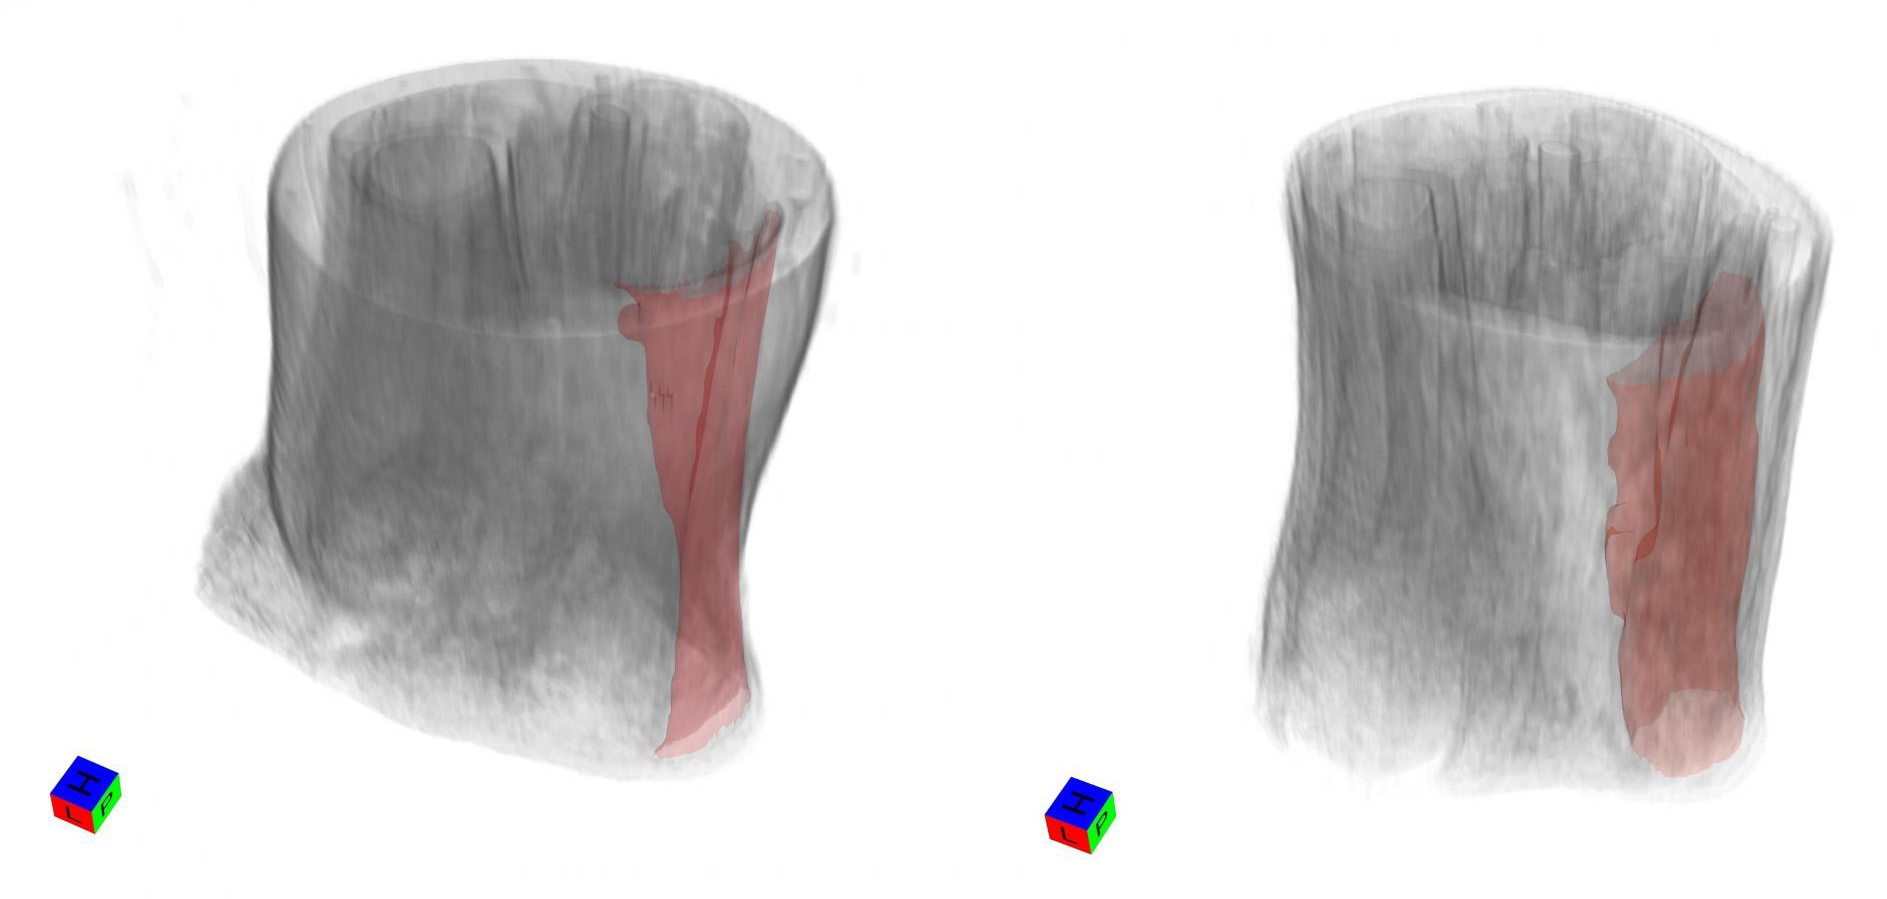
\includegraphics[width=\textwidth]{figures/Data_MRI_sample.png}
	\caption{Wizualizacja przykładowych danych RM w sekwencji PD dla zdrowego (po lewej) i gojącego się (po prawej) ścięgna Achillesa.}
	 \label{fig:MRI_sample}
\end{figure}
Obszar zajmowany przez tkankę ścięgnistą został oznaczony na czerwono. Należy zwrócić uwagę na różnicę w kształcie, która dla zdrowego przykładu jest zgodna z opisem anatomicznym ujętym w sekcji \ref{anatomia} natomiast dla przykładu chorego zawiera liczne deformacje.

Powyższe zbiory trójwymiarowe posłużyły do opracowania zbiorów dwuwymiarowych zawierających przekroje. W ten sposób udało się zwiększyć liczbę próbek wejściowych potrzebnych do szkolenia sieci neuronowych. Dane RM charakteryzują się wysoką anizotropią i ich rozdzielczość wynosi przykładowo 512$\times$512$\times$Z, gdzie $Z\in(10:50)$ (wyjątkiem jest sekwencja 3D FSPGR charakteryzująca się niższą anizotropią, jednak większą ilością artefaktów wynikających z szybkiego czasu akwizycji). Dlatego zbiory oparte o RM zostały stworzone w oparciu o przekroje osiowe 512$\times$512. W zależności od eksperymentów służących do doboru parametrów i komponentów metody wykorzystano:
\begin{itemize}
	\item powiększony zbiór treningowy RM -- zawiera przekroje osiowe ze wszystkich badań (z wyłączeniem pacjentów testowych) realizowanych wszystkimi sekwencjami. Dodatkowo liczba przekroi została powiększona poprzez zastosowanie transformacji odbicia lustrzanego i w przypadku chorych przykładów 10 obrotów w zakresie od -10 do 10 stopni. Finalnie zbiór zawiera 234.502 przekrojów oznaczonych jako zdrowych i 277.208 oznaczonych jako chorych.
	\item ograniczony zbiór treningowy RM -- zawiera przekroje osiowe ze zbioru oznaczonych 44 pacjentów jedynie w sekwencji T2 $^\ast$ GRE TE\_MIN (18.863 próbek).
	\item zbiór testowy -- zawiera przekroje pochodzące z danych zebranych dla 4 testowych pacjentów.
	\item zbiór PCA --
\end{itemize}

\subsubsection{Ultrasonografia:}
W przypadku danych Ultrasonografii stosowano się do identycznych odstępów czasowych, co w przypadku badań RM i akwizycji poddano tych samych pacjentów. Z przyczyn praktycznych zmniejszyła się jedynie grupa odniesienia, która w tym przypadku wyniosła 18-stu zdrowych ochotników. Badania zrealizowano z wykorzystaniem aparatu GE 3D high-resolution Voluson E8 Expert z liniową sondą (5--18 MHz). Jako dane wejściowe wykorzystano informacje z trybu B (zob. \ref{USG}), których ostateczna liczba wyniosła 565 3D skanów. 

Dane USG są zbliżone do izotropowych dlatego utworzono zbiory zarówno w oparciu o przekroje w płaszczyźnie osiowej jak i strzałkowej:
 \begin{itemize}
 	\item zbiór treningowy USG (strzałkowy) -- zawiera 253.639 2D przekrojów w płaszczyźnie strzałkowej, w tym 245.366 pochodzących od chorych 44 pacjentów oznaczonych przez radiologa i 8.273 pochodzących od zdrowych ochotników.
 	\item zbiór treningowy USG (osiowy) -- zawiera 467.548 2D przekrojów w płaszczyźnie osiowej, w tym 450.816 pochodzących od chorych 44 pacjentów oznaczonych przez radiologa i 16.732 pochodzących od zdrowych ochotników. 
 \end{itemize}

Wizualizacja przykładowych danych USG znajduje się na Rys. \ref{fig:US_sample}
\begin{figure}[h!]
	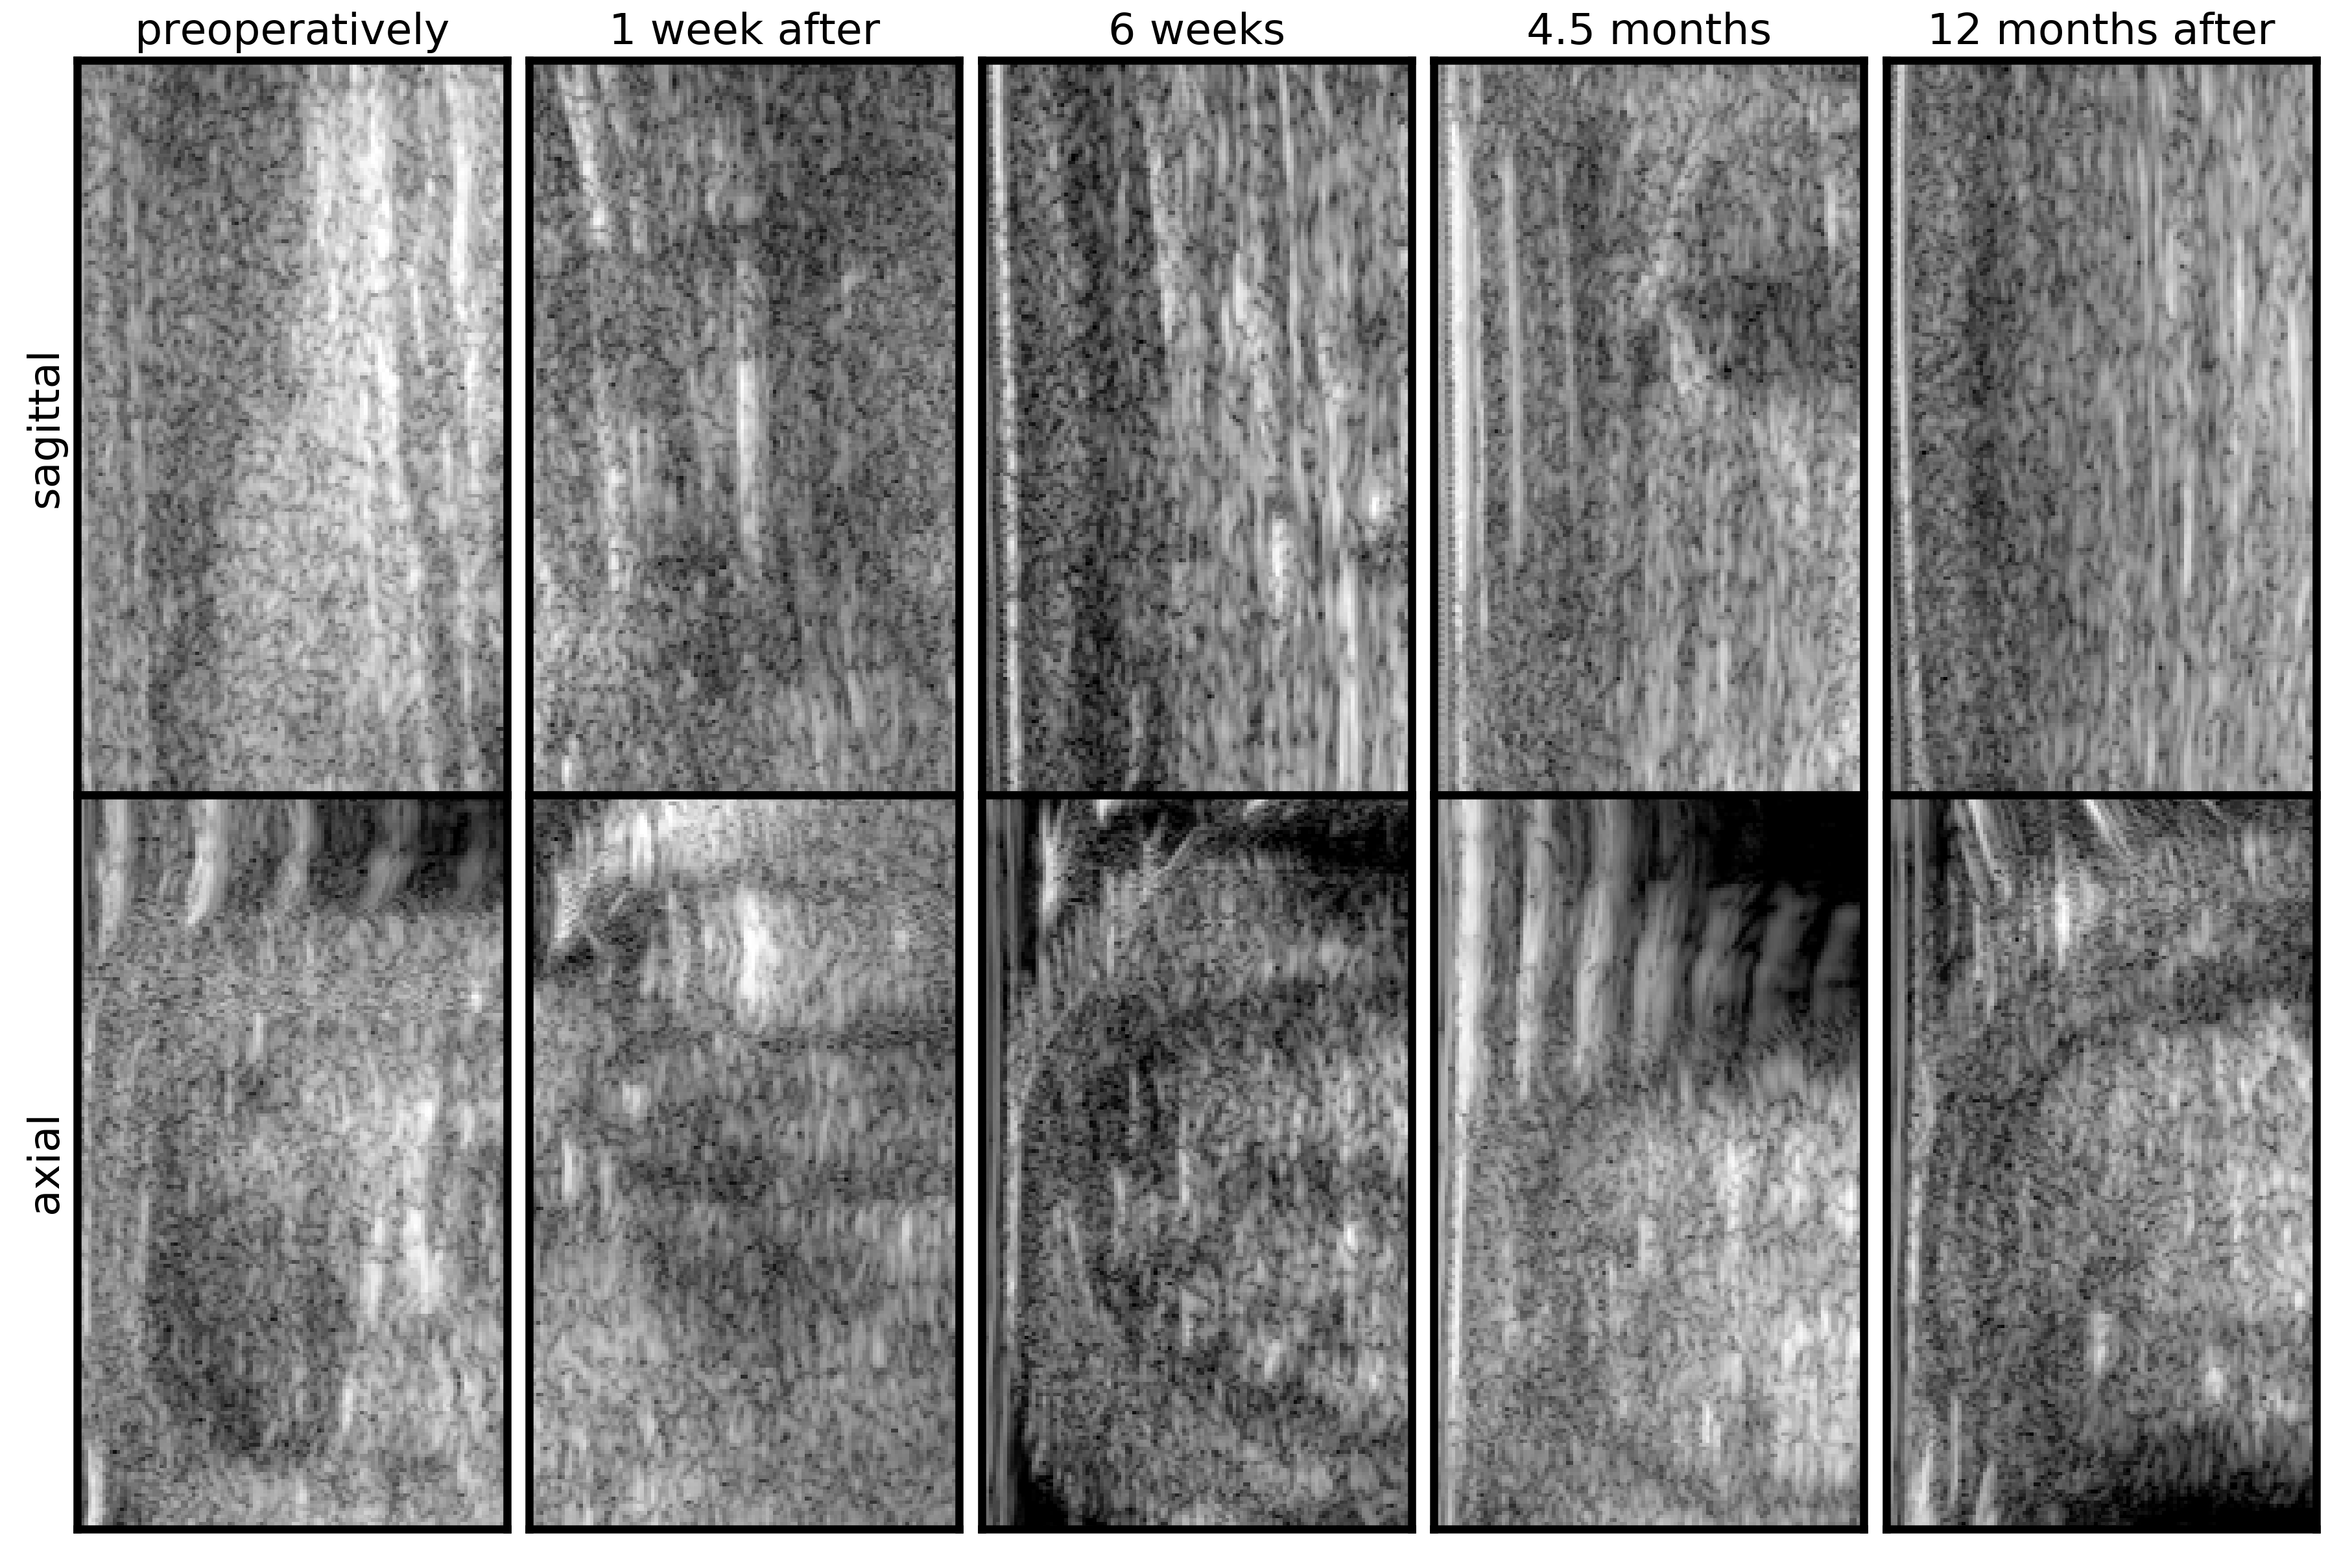
\includegraphics[width=\textwidth]{figures/Data_US_sample.png}
	\caption{Wizualizacja przykładowych danych USG w kolejnych tygodniach po zszyciu ścięgna w przekrojach osiowych i strzałkowych.}
	\label{fig:US_sample}
\end{figure}

Szczegółowa analiza załączonych obrazów może być wykonana jedynie przez specjalistę radiologa, jednak w ogólności można zaobserwować ułożenie włókien ścięgnistych na przekrojach strzałkowych i teksturę oraz tkanki otaczające ścięgno na przekrojach osiowych.
 

\subsection{wzorzec odniesienia}

Do stworzenia wzorca odniesienia, w ramach projektu START, została powołana specjalna grupa robocza składająca się z eksperta radiologa, specjalistów ortopedów i ekspertów od komputerowo wspomaganej diagnostyki. Celem grupy było opracowanie ilościowego opisu, który odzwierciedla elementy, na podstawie których radiolog podejmuje subiektywną opinię. W wyniku prac stworzono zestaw sześciu parametrów oceniany w skali 0--7 opisujący proces gojenia się ścięgna Achillesa widoczny w obrazach RM i Ultrasonografii:

\begin{enumerate}
	\item Uszkodzenia śródścięgniste (SCT od ang. \textit{Structural changes within the tendon}) -- informuje o spójności włókien w obszarze ścięgna. Zawiera się w ROI. Ocena wykonywana zarówno w płaszczyznie osiowej jak i strzałkowej. 0 – całkowity brak uszkodzeń, 1 – bardzo małe uszkodzenia. 2 – małe uszkodzenia, 3 – uszkodzenia średniej wielkości , 4 – dość duże uszkodzenia. 5 – duże uszkodzenia, 6 - bardzo duże uszkodzenia, 7 - ekstremalnie duże uszkodzenia.
	\item Pogróbienie ściegna (TT od ang. \textit{Tendon thickening} -- najgrubsze miejsce w kierunku strzałkowym na widoczne na przekroju osiowym. Zawiera się w ROI. 0 – całkowity brak pogrubienia (3mm-5mm), 1 – bardzo małe pogrubienie - 6mm, 2 – małe pogrubienie - 9mm, 3 – średnie pogrubienie- 12mm, 4 –  dość duże pogrubienie -15mm, 5 duże pogrubienie - 18mm, 6 – bardzo duże pogrubienie - 21mm, 7 – ekstremalnie duże pogrubienie – 24mm.
	\item Ostrość granic ścięgna/rozgraniczenie (STE od ang. \textit{Sharpness of the tendon edges})-- informuje o jakości granicy między tkankami ścięgnistymi i otoczeniem, w szczególności, czy brzeg jest fraktalny. Oceniane na zewnątrz ścięgna w płaszczyznie osiowej. 0 – bardzo duża (idelana) ostrość, 1 – duża ostrość, 2 – dość duża ostrość, 3 – średnia ostrość, 4 – mała ostrość, 5 – bardzo mała ostrość, 6 – minimalna ostrość, 7 – całkowicie nieostre.
	\item Obrzęk ścięgna (TE od ang. \textit{Tendon edema}) -- informuje o anomaliach w gromadzeniu się płynów w obszarze ścięgna. Zawiera się w ROI i jest oceniany na przekrojach osiowych. 0 – całkowity brak obrzęku, 1 – bardzo mały obrzęk, 2 – mały obrzęk, 3 – obrzęk średniej wielkości, 4 – dość duży obrzęk, 5 – duży obrzęk. 6 – bardzo duży obrzęk, 7 - ekstremalnie duży obrzęk.
	\item Jednorodność ścięgna (TU od ang. \textit{Tendon uniformity}) -- informuje o prawidłowej teksturze poszczególnych przekrojów osiowych jak i podobieństwu sąsiednich, mierzonym w płaszyznie strzałkowej. Zawiera się w ROI. 0 – całkowity brak niejednorodności (jednorodne), 1 – bardzo małe niejednorodności, 2 – małe niejednorodności, 3 – niejednorodności średniej wielkości, 4 – dość duże niejednorodności, 5 – duże niejednorodności, 6 – bardzo duże niejednorodności, 7 –  ekstremalnie duże niejednorodności. 
	\item Obrzęk tkanek (TisE od ang. \textit{Tissue edema}) -- informuje o powiększonym przedziale powięziowym ścięgna. 0  – całkowity brak obrzęku, 1 – bardzo mały obrzęk, 2 – mały obrzęk, 3 – obrzęk średniej wielkości, 4 – dość duży obrzęk, 5 – duży obrzęk. 6 – bardzo duży obrzęk, 7 - ekstremalnie duży obrzęk.
\end{enumerate}

Obrazowania 3D zostały opisane przez eksperta radiologa przy użyciu ankiety zawierającej powyższe parametry. W ramach projektu START udało się zgromadzić opisy dla badań RM i USG 48 pacjentów (480 badań). 4 z nich zostało losowo wydzielonych na początku eksperymentów jako pacjenci testowi. Szczegółowy opis eksperymentów znajduje się w kolejnej sekcji.

\section{Eksperymenty}

W tej sekcji zestawiono eksperymenty mające na celu dobór poszczególnych komponentów i parametrów finalnej metody. W pierwszej kolejności zostało opisane badanie dotyczące szkolenia sieci neuronowych celem rozróżnienia ścięgien zdrowych od tych po zerwaniu (chorych). Następnie zaprezentowano badanie dotyczące obliczania wektora cech na wyjściu sieci neuronowej i redukcji jego wymiarowości. W kolejnej części przedstawiono wybór sekwencji RM, które stanowiły dane wejściowe do proponowanego w tej pracy algorytmu. Finalnie, w dwóch ostatnich podsekcjach opisano dobór optymalnego zestawu mieszanki cech ekstrahowanych z użyciem sieci neuronowej i metod przetwarzania obrazów oraz fuzję cech z wykorzystaniem meta-regresji.  


\subsection{Rozróżnienie ścięgna zdrowego i po zerwaniu}

W tym badaniu porównane zostały współczesne architektury sieci neuronowych w zadaniu klasyfikacji binarnej, rozróżniającej obrazy zdrowego od chorego ścięgna. W porównaniu uwzględniono topologie AlexNet (zob. \ref{AlexNet}), GoogLeNet InceptionV3 (zob. \ref{googlenet}) i ResNet-18 (zob. \ref{resnet}). W celu doboru hiperparametrów i optymalizacji parametrów sieci zastosowano szkolenie z wykorzystaniem kroswalidacji z podziałem na 5 segmentów (zob. \ref{sec-overffiting}). W każdym z 5 cykli, 3 segmenty były wykorzystane do treningu, 1 do walidacji i 1 do finalnych testów. Do celów tego badania wykorzystano powiększony zbiór treningowy RM. Wyniki z testów zebrano w Tab. \ref{cross-validation}.
%\vspace{-10px}
\begin{table}[h!]
	\setlength{\tabcolsep}{14pt}
	\centering
	\caption{Wyniki szkolenia sieci neuronowych z wykorzystaniem kroswalidacji z podziałem na 5 segmentów dla problemu klasyfikacji obrazów zdrowego i chorego ścięgna.}
	\label{cross-validation}
	\begin{tabular}{l | l | l | l | l }
		%\hline
		 & Average   & Min   & Max   & SD   \\ \hline \hline
		AlexNet   & 99.19 & 99.15 & 99.24 & 0.04 \\ \hline
		ResNet-18 & 95.98 & 92.78 & 99.04 & 2.5  \\ \hline
		GoogleNet & 99.83 & 99.68 & 99.91 & 0.1  \\ %\hline
	\end{tabular}
\end{table}
%\vspace{-10px}

Dla wszystkich architektur sieci, wyniki dokładności klasyfikacji najlepszych modeli osiągnęły wartość powyżej 99\%. Niemniej jednak w przypadku architektury ResNet-18 najgorszy model klasyfikował z dokładnością 92.78\%, co przełożyło się równiez na najgorszy średni wynik 95.98\%. Fakt ten może wskazywać na tendencje do nadmiernego dopasowywania się architektury ResNet-18 wynikający z niedoboru liczby danych wejściowych w odniesieniu do liczby optymalizowanych parametrów w warstwach konwolucyjnych.

Dla wszystkich trzech architektur porównano również czasy szkolenia się dla zadanego problemu. Na Rys. \ref{fig:training_times} zestawiono łączny czas 5 iteracji procesu kroswalidacji.

\begin{figure}[h!]
	\includegraphics[width=\textwidth]{figures/TrainingtimesChart.png}
	\caption{Porównanie czasów treningu architektur na dwóch architekturach GPU: Pascal i Volta.}
	\label{fig:training_times}
\end{figure}

Porównano dwie architektury GPU tj. starszą Pascal P100 i nowszą Volta V100, zaprezentowaną w 2017 roku, charakteryzującą się udoskonalonym osobnym układem optymalizowanym pod kątem operacji tensorowych realizowanych w warstwach splotu. Do szkolenia wykorzystano framework Caffe. Można zaobserwować, że wykorzystanie nowszej architektury GPU dało rezultaty około dwukrotnego przyspieszenia czasu szkolenia w przypadku AlexNet i ResNet oraz około 30\% w przypadku GoogLeNet. AlexNet zawiera najmniej warstw konwolucyjnych i optymalizowaną implementację klasyfikatora. Szkolenie tej architektury zajęło mniej niż jedną godzinę na GPU Volta. Dla porównania, sieci z bardziej skomplikowaną topologią tj. ResNet-18 i GoogLeNet charakteryzują się odpowiednio czasami szkolenia w okolicach 20 i 48 godzin. 

Biorąc pod uwagę zestawienie wyników dokładności klasyfikacji i czasu szkolenia najlepszą architekturą okazała się sieć AlexNet, dlatego została ona wybrana do realizacji kolejnych eksperymentów. Należy również wspomnieć, że rezultaty wnioskowania mogą wciąż być poprawione. Dla przykładu, uzupełniające badanie dotyczące możliwości fuzji sieci AlexNet i ResNet-18 zostało opublikowane przez autora tej pracy w Acta of Bioengineering and Biomechanics \cite{Kapinski19}. Wyniki mogą być również poprawione w wyniku analizy lokalizacji przekrojów w przestrzeni trójwymiarowej, a w szczególności poprzez uwzględnienie, że częściej przekroje oddalone od miejsca zerwania bardziej przypominają tkanki zdrowe. W tym zakresie można np. zastosować metody logiki rozmytej lub miękkiej klasyfikacji (zob. []). Niemniej jednak, z uwagi na wysokie wyniki dokładności możliwie prostego podejścia w tej pracy autor nie decyduje się na dalsze usprawnienia kosztem komplikacji algorytmu. Ewentualne anomalie i wyniki odosobnione zostaną wyeliminowanie poprzez zastosowanie średniej trymowanej w zaproponowanej metryce $H$ (zob. \ref{ecq:H}).

\subsection{Obliczanie i redukcja wymiarowości wektora cech}

Celem tego eksperymentu jest znalezienie zredukowanego wektora cech pochodzących z wyjścia sieci neuronowej (cechy DL), który zawierałby możliwie dużo informacji z oryginalnego zbioru. W tym celu z oryginalnej architektury AlexNet została wydzielona część ekstraktora cech oraz pierwsza warstwa typu fully-connected (zob. Rys. \ref{AlexNetTopology}). Parametry ekstraktora cech zostały zachowane dobrane zgodnie z najlepszym modelem z uprzednio opisanego eksperymentu binarnej klasyfikacji. Warstwa fully-connected umożliwia wstępne pogrupowanie cech obrazowych, a jednocześnie nie dywersyfikuje ich w stopniu jaki robi to pełna sieć. Wykorzystując zbiór danych PCA, została przeprowadzona analiza czynników głównych (zob. \ref{DimReduction}), gdzie pojedyncza obserwację stanowił wektor 4096 cech DL przekrojów 10 pacjentów w poszczególnych tygodniach rehabilitacji. Dzięki temu analiza umożliwiła redukcję wymiarowości i jednocześnie zwiększenie rozróżnienia między obserwacjami w poszczególnych krokach czasowych. Porównanie poziomu wariancji zachowywanej przez różną liczbę czynników głównych zebrano w Tab. \ref{PCA-results}.
\begin{table}[h!]
 \setlength{\tabcolsep}{12pt}
 \centering
 \caption{Rezultaty PCA dla 1, 10 i 200 pierwszych czynników głównych.}
 \label{PCA-results}
 \begin{tabular}{l|l|l|l}
 \hline
 & PC1 & PC1-PC10 & PC1-PC200 \\ \hline
 Zachowany poziom wariancji & 50.2\% & 90.8\%   & 98.8\% \\ \hline 
 \end{tabular}
 \end{table}

Rezultaty wskazują, że 4096 cech DL może być zredukowanych do jednego wyjścia zachowując przy tym ponad 50\% poziomu wariancji. Odpowiednio 10 czynników zapewnia poziom powyżej 90\%, a 200 czynników poziom bliski 99\%. 

W celu lepszego zrozumienia informacji zachowywanej przez użytą transformację PCA dla wszystkich użytych w tej pracy sekwencji i modalności RM zostały zwizualizowane trendy PC1 dla uśrednionych wyników z 10 pacjentów. Przy czy wynik dla poszczególnego badania 3D wyliczono modyfikując równanie:  

\begin{equation}
H = TM(PC1(x_1), PC1(x_2),..., PC1(x_n))
\end{equation}

Na Rys. \ref{fig:H} przedstawiono otrzymane krzywe.

\begin{figure}[h!]
	\centering
	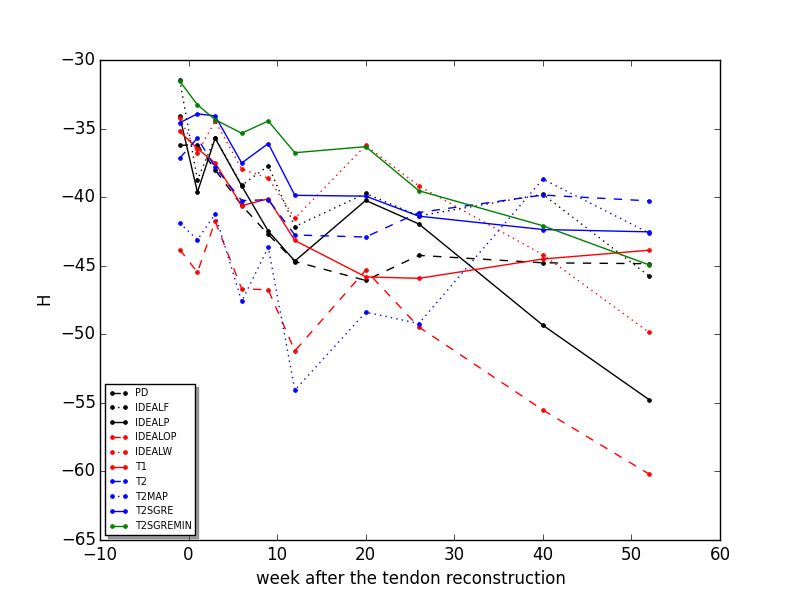
\includegraphics[width=0.8\textwidth]{figures/H_PC1.png}
	\caption{Porównanie krzywych dla 10 modalności RM reprezentujących średnią $H$ z 10 pacjentów.}\label{fig:H}
\end{figure}

Oprócz sekwencji T2 mapping wszystkie sekwencje i modalności pokazują malejący trend rozumiany jako ujemna różnica pomiędzy wartością końcową i początkową okresu rehabilitacji. Odmienny trend T2 mapping może być spowodowany faktem, że dla tej sekwencji dane były zbierane we wszystkich 8 różnych poziomach sygnały T2. W związku z czym w obrazach pojawiają się próbki silnie zaszumione i zniekształcone. Dopiero głębsza analiza związana np. z wyliczaniami na podstawie aproksymacji sygnału może skutkować poprawą rezultatów \cite{Regulski2017}. 

W pozostałych przypadkach otrzymane trendy odpowiadają naturze procesu gojenia i kolejnym jego etapom. Na początku procesu zmiany są bardzo wyrazne w badaniach obrazowych, co zmniejsza się na kolejnych etapach. Dynamika i fluktuacje zależą również od indywidualnych cech pacjenta oraz innych czynników jak przestrzeganie zaleceń, co do rehabilitacji, diety i aktywności pacjenta. Wynikiem tego eksperymentu jest zatem metoda redukcji wymiarowości przestrzeni cech DL z jednoczesnym zachowaniem istotnej informacji z punktu widzenia oceny procesu gojenia. 


\subsection{Wybór sekwencji rezonansu magnetycznego}

Z uwagi na opisany w Sekcji \ref{RM} tor akwizycji danych RM zwiększanie liczby sekwencji odbywa się kosztem wydłużenia czasu badania pacjenta. W skrajnym przypadku, takim jak pozyskanie wszystkich 10 omawianych sekwencji, czas ten wynosi około 1 godziny, co stanowi praktyczne ograniczenie opracowywanej metody. Dlatego celem tego eksperymentu jest wybór protokołu zawierającego minimalną liczbę sekwencji umożliwiających przy użyciu opracowywanej metody skuteczną ocenę procesu gojenia. Prace podzielono na dwa zakresy tj. analizę wizualną i ilościową.

\subsubsection{Analiza wizualna:} W ramach wstępnej analizy, wartości danych ze wszystkich sekwencji i modalności zebranych od pacjentów zostały zakumulowane w postaci znormalizowanych histogramów i przedstawione na Rys. \ref{fig:Hists}.

\begin{figure}[h]
	\centering
	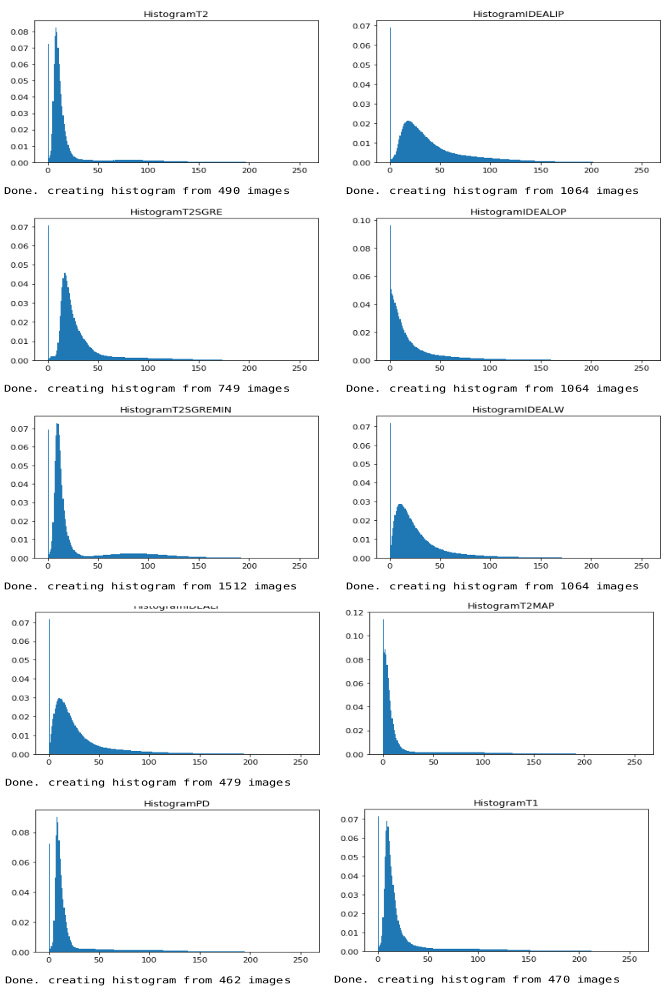
\includegraphics[width=0.6\textwidth]{figures/Hists.png}
	\caption{Znormalizowane histogramy dla 10 sekwencji RM.}\label{fig:Hists}
\end{figure}

W celu porównania, dane zostały przeskalowane aby wartość całki była równa 1, a zakres <0; 255>. Widoczne we wszystkich przypadkach maksima w zerze są naturalnie wynikiem tła, które stanowi powietrze. Analizując pozostałe wartości można wyróżnić następujące 3 grupy:

\begin{enumerate}
	\item Bez maksimum poza zerem -- sekwencja T2 mapping i modalność Out Phase Ideal. W pierwszym przypadku jest to konsekwencja wspomnianej już w poprzednim eksperymencie występowania danych ze wszystkich 8 próbek sekwencji, czyli również tych mierzonych przy prawie zerowym sygnale T2, silnie zaszumionych z licznymi wartościami bliskimi zeru. W drugim przypadku na granicach wody i tłuszczu występuje często silne rozmycie (tzw. \textit{artefakt czarnego atramentu}), co również zwiększa liczbę wartości bliskich zeru.
	\item Z jednym maksimum poza zerem -- pozostałe modalności 3D FSPGR oraz sekwencje: PD, T1 zależne, T2 zależne, T2 $^\ast$ GRE. Przypadek najczęściej występujący. Wartości sygnału zależą od tkanek dominujących w obrazowanym elemencie.
	\item Z dwoma maksimami poza zerem -- sekwencja T2 $^\ast$ GRE TE\_MIN. Jako jedyna posiada drugie maksimum lokalne, co może wskazywać na zwiększoną czułość na wzorce zawarte w danych.  
	
\end{enumerate}
%dlaczego wyrzucamy 3DFSPGR?
Na podstawie powyższej, zgrubnej analizy można wyłączyć z dalszych badań pierwszą grupę sekwencji, z uwagi na możliwość występowania wysokiego szumu w sygnale oraz artefaktów. Zdecydowanie wyróżniająca się sekwencją jest T2 $^\ast$ GRE TE\_MIN. Żeby lepiej zrozumieć istotność występowania drugiego maksimum na Rys. \ref{fig:protocol_comp} zestawiono przykład rekonstrukcji danych z wykorzystaniem sekwencji z obu analizowanych dalej grup. 

 \begin{figure}[h]
 	\centering
 	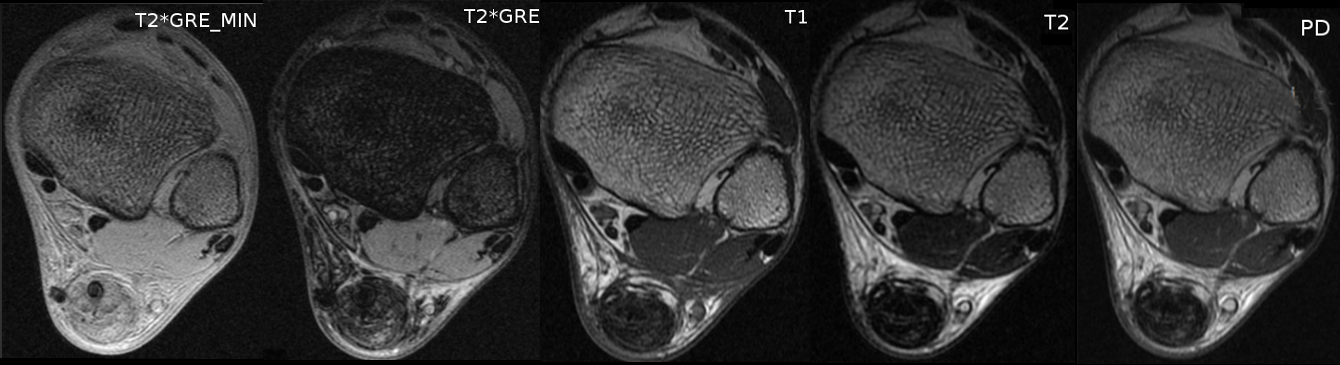
\includegraphics[width=0.95\textwidth]{figures/Protocol_comparison.png}
 	\caption{Porównanie sekwencji RM ilustrujących proces gojenia się ścięgna Achillesa w 12 tygodniu po rekonstrukcji.}\label{fig:protocol_comp}
 \end{figure}

Główna różnica w rekonstruowanych przy pomocy powyższych danych obrazów pochodzi z różnicy w odcieniach szarości w obszarze ścięgna. Obrazy w dwunastym tygodniu procesu gojenia się, rekonstruowane przy pomocy sekwencji z grupy (2), charakteryzują się wartościami w obszarze ścięgna bliskimi zeru. Jedynie na obrazach rekonstruowanych z wykorzystaniem danych z T2 $^\ast$ GRE TE\_MIN obszar ścięgna jest jaśniejszy. W celu lepszego zobrazowania różnicy na Rys. \ref{fig:T2comp} przedstawiono próbki zrekonstruowane w kolejnych krokach czasowych.

\begin{figure}[h]
	\centering
	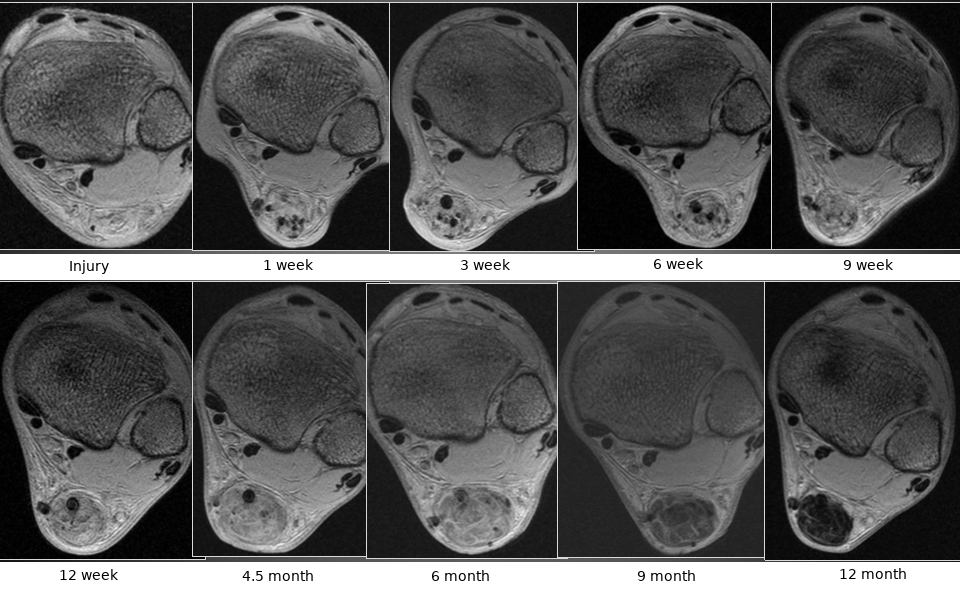
\includegraphics[width=0.95\textwidth]{figures/T2gremin.png}
	\caption{Proces gojenia się ścięgna Achillesa widoczny w obrazach zrekonstruowanych na podstawie danych z sekwencji T2 $^\ast$ GRE TE\_MIN}\label{fig:T2comp}
\end{figure}

Analiza wizualna wskazuje, że różnice w odcieniach szarości mogą wspomóc radiologów w skutecznej interpretacji stopnia wygojenia się tkanek ścięgnistych. Wartości w obszarze ścięgna są jasne na początku i ciemnieją z czasem. Fakt ten może wynikać z czasu relaksacji T2, który dla sekwencji T2 $^\ast$ GRE TE\_MIN jest bardzo krótki. Stąd autor tej pracy stawia hipotezę, że sekwencja ta jest bardzo czuła na ilość krwi dostarczanej do tkanek. Zmiany w tym zakresie na przestrzeni całego procesu gojenia się ścięgna uwidaczniają się w postaci silnie rozróżnialnych zmian w odcieniach szarości w obszarze ścięgna, co z kolei jest również wartościową informacją z uwagi na zastosowane w tej pracy metody sztucznej inteligencji i przetwarzania obrazów. Powyższe obserwacje i wnioski posłużyły jako punkt startu dla przedstawionych poniżej analiz ilościowych.

\subsubsection{Analiza ilościowa:} W ramach tego badania ilościowo porównano wyniki automatycznej oceny procesu gojenia się ścięgna Achillesa przy użyciu danych (1) tylko z sekwencji T2 $^\ast$ GRE TE\_MIN oraz (2) danych z sekwencji T2 $^\ast$ GRE TE\_MIN oraz PD i T2 $^\ast$ GRE. Wybierając sekwencję T2 $^\ast$ GRE TE\_MIN kierowano się wynikami analizy wizualnej, natomiast dobór pozostałych dwóch sekwencji, poza analizą wizualną i wiedzą dziedzinową, był umotywowany oceną stopnia korelacji. W tym celu w Tab. \ref{tab:inter-protocol-corr} zestawiono porównanie sekwencji z grupy (2) -- bez modalności 3DFSPGR.

\begin{table}[h]
	\centering
	\setlength{\tabcolsep}{12pt}
	\caption{Korelacja sekwencji PD, T1, T2 and T2$^\ast$ GRE MRI. Wyniki oznaczone pogrubieniem są istotne statystycznie z p $<$ 0.01.}
	\label{tab:inter-protocol-corr}
	\begin{tabular}{l||c|c|c|c}
		%\hline
		& PD & T1 & T2 & T2$^\ast$GRE \\ \hline \hline
		PD & 1.00 & \textbf{0.96} & \textbf{0.90} & \textbf{0.89} \\ \hline
		T1 & \textbf{0.96} & 1.00 & \textbf{0.85} & \textbf{0.92} \\ \hline
		T2 & \textbf{0.90} & \textbf{0.85} & 1.00 & 0.71 \\ \hline
		T2$^\ast$GRE & \textbf{0.89} & \textbf{0.92} & 0.71 & 1.00  %\hline
	\end{tabular}
	%\vspace{-0.5cm}
\end{table} 

Jako dane do obliczeń korelacji wybrano informacje z $H$ (zob. \ref{ecq:H}) zawierającą wartości zredukowanej do pierwszego czynnika głównego przestrzeni cech.  Uwzględniając wyniki istotne statystycznie, wśród najbardziej skorelowanych sekwencji znalazły się T1 i PD. Z tej pary PD jest rutynowo używany przez radiologów do zadanego w tej pracy problemu dlatego został uwzględniony w kolejnych testach. PD najmniej koreluje z T2$^\ast$GRE, stąd końcowa decyzja.

W celach porównań, wykorzystano ponownie zredukowaną przestrzeń czynników głównych i wykonano szereg obliczeń stopnia gojenia się ścięgna stosując poniższą metrykę: 

\begin{equation}
H_{2} = \alpha + \sum_{i=1}^{3}\beta_{i}X_{i} + \sum_{i=1}^{3}\gamma_{i}X_{i}^{2} +
\sum_{\substack{i, j = 1\\ i < j}}^{3}\lambda_{i,j}X_{i}X_{j}
\end{equation}

gdzie $X_i = TM(PC_n(x_1), PC_n(x_2),..., PC_n(x_n))_{i}$ to kolejne predyktory, $TM$ to średnia trymowana z marginesami 2.5\%, $PC_n(x_k)$ to $n$-ty czynnik główny otrzymany przy wnioskowaniu sieci dla przekroju osiowego $x_k$, gdzie $k$ jest indeksem przekroju danego protokołu w trójwymiarowym badaniu RM.

W szczególności wyliczono różne modele regresji poczynając od liniowej, gdzie ($\gamma_{i}=0, \lambda_{i}=0$), przez nieliniową stopnia drugiego ($\lambda_{i}=0$) oraz z kombinacją czynników. W przypadku liniowym wykorzystano od 1 do 10 czynników głównych natomiast w przypadku nieliniowym wykorzystano tylko dwa pierwsze z uwagi na zabieganie nadmiernemu dopasowaniu się modelu. Powyższe modele zestawiono z modelem liniowej regresji wytrenowanym jedynie na danych z T2 $^\ast$ GRE TE\_MIN. Do obliczenia współczynników regresji zastosowano zbiór pacjentów treningowych. Natomiast w celach porównań zestawiono wyniki dla pacjentów testowych, a dokładniej wyliczono metryki średniego błędu absolutnego (MAE od ang.\textit{mean absolute error}), maksymalnego błędu absolutnego (MAX-AE od ang. \textit{max. absolute error}) i średniej korelacji obliczonej z wykorzystaniem trasformacji Z-fishera (Corr od ang. \textit{correlation}). Rezultaty znajdują się w Tab. \ref{tab:H_testset}.

\begin{table*}[t]
	\caption{Porównanie różnych modeli regresji.}
	\scriptsize
	\begin{center}
		\begin{tabular}{lc||c|c|c|c|c|c}
			\textbf{Model} & & \textbf{SCT} & \textbf{TT} & \textbf{STE} & \textbf{TE} & \textbf{TU} & \textbf{TisE}\\ 
			
			\hline
			model\_PC1 & MAE & 1.26 $\pm$ 0.44 & \textbf{0.71} $\pm$ 0.12 & \textbf{0.7} $\pm$ 0.16 & 0.97 $\pm$ 0.26 & \textbf{0.92} $\pm$ 0.29 & 0.99 $\pm$ 0.25\\
			&MAX-AE &3.53&2.49&1.91&\textbf{2.34}&2.2&2.47\\
			&Corr &0.58&0.47&-0.07&0.60&\textbf{0.56}&0.58\\
			
			\hline
			model\_PC1\_2 & MAE & 1.28 $\pm$ 0.47 & 0.74 $\pm$ 0.13 & 0.71 $\pm$ 0.19 & 0.98 $\pm$ 0.26 & 0.94 $\pm$ 0.3 & 1.02$\pm$ 0.28\\
			&MAX-AE &3.64&2.56&1.94&2.98&2.35&2.9\\
			&Corr &0.53&0.30&0.02&0.51&0.41&0.60\\
			
			\hline
			model\_PC1\_3&MAE & 1.43 $\pm$ 0.58 & 0.71 $\pm$ 0.13 & 0.73 $\pm$ 0.23 & 1.02 $\pm$ 0.31 & 1.05 $\pm$ 0.36 & 1.07 $\pm$ 0.37\\
			&MAX-AE &3.99&2.49&1.98&3.2&2.96&3.02\\
			&Corr &0.48&0.36&0.03&0.50&0.29&0.62\\
			
			\hline
			model\_PC1\_4&MAE & 1.39 $\pm$ 0.53 & 0.72 $\pm$ 0.09 & 0.8 $\pm$ 0.22 & 1.01 $\pm$ 0.3 & 1.02 $\pm$ 0.33 & 1.06 $\pm$ 0.37\\
			&MAX-AE &3.56&\textbf{2.4}&2.17&3.2&2.61&3.13\\
			&Corr &0.54&0.37&0.17&0.52&0.38&\textbf{0.68}\\
			
			\hline
			model\_PC1\_5&MAE & 1.35$\pm$ 0.5 & 0.79$\pm$0.06 &0.8$\pm$0.25 &0.99$\pm$0.26 &1.01$\pm$0.26 &1.1$\pm$0.29\\
			&MAX-AE &3.45&2.69&2.39&3.21&2.55&2.88\\
			&Corr &0.49&0.31&0.22&0.52&0.30&0.60\\
			
			\hline
			model\_PC1\_6&MAE & 1.32$\pm$0.49 & 0.78$\pm$0.05 &0.8$\pm$0.25& 0.97$\pm$0.29 & 0.98$\pm$0.24 &1.11$\pm$0.25\\
			&MAX-AE &\textbf{3.3}&2.64&2.21&3.12&2.6&2.8\\
			&Corr &0.53&0.33&0.21&0.56&0.38&0.56\\
			
			\hline
			model\_PC1\_7&MAE &$1.33\pm{0.5}$&$0.78\pm{0.07}$&$0.82\pm{0.26}$&$1.03\pm{0.31}$&$0.99\pm{0.26}$&$1.14\pm{0.29}$\\
			&MAX-AE &3.34&2.75&2.41&3.17&2.63&2.69\\
			&Corr &0.53&0.33&0.21&0.54&0.30&0.57\\
			
			\hline
			model\_PC1\_8&MAE & 1.35$\pm$0.49 & 0.77$\pm$0.08& 0.81$\pm$0.26&1.02$\pm$0.31& 0.99$\pm$0.28 & 1.14$\pm$0.27\\
			&MAX-AE &3.41&2.58&2.47&3.13&2.65&2.75\\
			&Corr &0.54&0.37&0.19&0.53&0.25&0.55\\
			
			\hline
			model\_PC1\_9&MAE & 1.38$\pm$0.48 & 0.74$\pm$0.09 & 0.76$\pm$0.27 & 1.03$\pm$0.28 & 1.02$\pm$0.3 & 1.12$\pm$0.27\\
			&MAX-AE &3.49&2.57&2.45&2.9&2.7&2.67\\
			&Corr &0.52&0.40&\textbf{0.25}&0.55&0.30&0.58\\
			
			\hline
			model\_PC1\_10&MAE & 1.37$\pm$0.49 & 0.74$\pm$0.11 & 0.76$\pm$0.27 & 1.04$\pm$0.27 & 1.03$\pm$ 0.29& 1.11$\pm$0.28\\
			&MAX-AE &3.46&2.42&2.52&2.92&2.67&2.68\\
			&Corr &0.50&0.38&0.24&0.54&0.29&0.59\\
			
			\hline
			model\_poly&MAE & 1.27$\pm$ 0.49 & 0.74$\pm$0.1 & 0.71$\pm$0.2 & 0.93$\pm$0.28 & 0.95$\pm$0.31 & 1.03$\pm$0.25\\
			&MAX-AE &3.62&2.6&1.96&2.83&2.29&2.87\\
			&Corr &0.53&0.34&0.11&\textbf{0.61}&0.37&0.58\\
			
			\hline
			model\_cross\_poly&MAE & 1.3$\pm$0.47 & 0.75$\pm$0.1 & 0.78$\pm$0.24 & 0.93$\pm$0.28 & 1.01$\pm$0.42 & 1.06$\pm$0.32 \\
			&MAX-AE &3.64&2.7&2.01&2.83&3.36&2.86\\
			&Corr &0.53&0.45&0.12&0.58&0.15&0.57\\
			\hline  \hline
			
			baseline& MAE & \textbf{1.24}$\pm$0.16 & 0.82$\pm$0.09 & 0.75$\pm$0.08 & 1.06$\pm$0.10 & \textbf{0.90}$\pm$0.09 & \textbf{0.96}$\pm$0.10 \\
			&MAX-AE & 3.54 & 2.46 & \textbf{1.82} & 2.70 & \textbf{2.13} & \textbf{2.18}\\
			&Corr   & \textbf{0.61} & \textbf{0.64} &-0.08 & 0.55 & 0.55 & 0.65\\
			\hline
		\end{tabular}
	\end{center}
	\label{tab:H_testset}
\end{table*}

Model prostej liniowej regresji wykorzystujący jedynie informacje z sekwencji T2 $^\ast$ GRE TE\_MIN był najskuteczniejszy w największej liczbie mierzonych parametrów tj. 8 z 18. 3 razy osiągnął najlepszy wynik w MAE i MAX-AE oraz dwukrotnie w Corr. Zatem dodawanie sekwencji jako danych wejściowych i komplikacje modelu skutkują nadmiernym dopasowaniem oraz pogorszeniem jakości automatycznej oceny. Należy również podkreślić, że akwizycja samej sekwencji T2 $^\ast$ GRE TE\_MIN dla omawianego problemu zajmuje około 5 min. podczas gdy wszystkich trzech sekwencji trwa około 12 minut na pacjenta. Podsumowując, na podstawie analizy wizualnej i jakościowej, jako dane wejściowe do kolejnych eksperymentów została wybrana sekwencja T2 $^\ast$ GRE TE\_MIN. 

\subsection{Optymalna konkatenacja cech}
\subsection{Fuzja z wykorzystaniem meta-regresji}



\section{Ocena procesu gojenia}

-- porównanie z end-to-end




%\subsection{Topologia sieci}
%\subsection{Redukcja wymiarowości}
%\subsection{Miara wygojenia}
